\mysubsectionformatted{Transazioni e Stati transazionali}
\myparagraph{
    Una \textbf{Transazione} è un'unità di lavoro i cui compiti devono essere completati tutti con successo,
    oppure nessuno di essi deve essere completato. 

    Quando lavoriamo su oggetti persistenti (li inseriamo, cancelliamo o aggiorniamo), questi non vengono aggiornati
    subito nel database, bisogna quindi eseguire un'operazione di commit esplicita.
    Possiamo definire \textbf{3 luoghi} in cui possono trovarsi gli oggetti persistenti:
    \begin{enumerate}
        \item nell'applicazione
        \item nel database
        \item nella cache
    \end{enumerate} 

    Si possono anche definire gli \textbf{stati} associati agli oggetti persistenti:
    \begin{enumerate}
        \item \textbf{New}: appena creato e non ancora presente nel DB
        \item \textbf{Old}: recuperato dal DB (quindi creato in precedenza) 
        \item \textbf{Clean}: non modificato
        \item \textbf{Dirty}: modificato
        \item \textbf{Deleted}: cancellato
    \end{enumerate}

    \setcounter{figure}{0}

    \begin{figure}[h]
        \caption{Diagramma degli Stati}
        \centering
        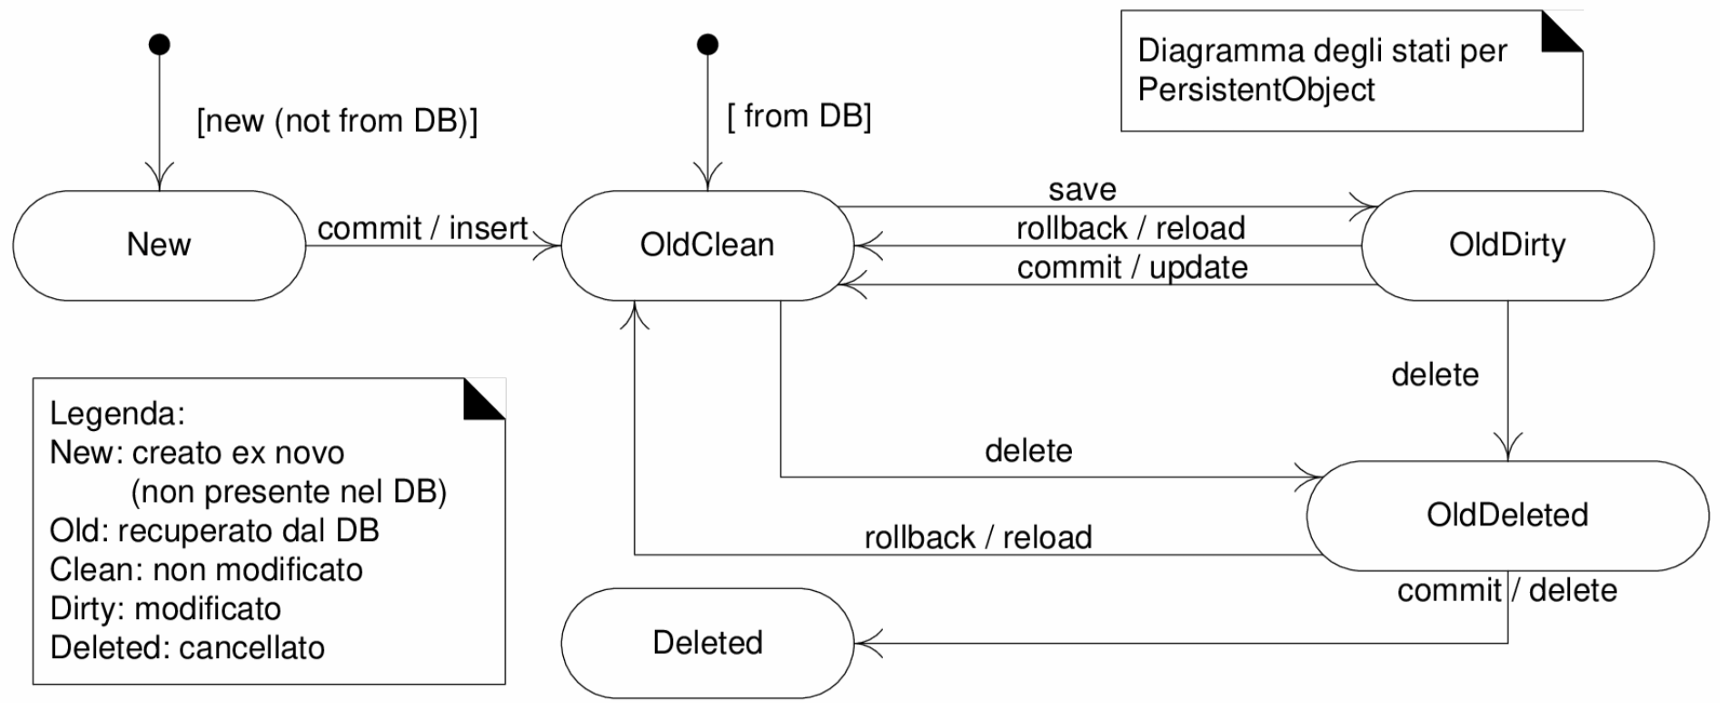
\includegraphics[scale=0.27]{Esercitazione - Design Patterns/Diagramma degli Stati.png}
    \end{figure}
    \textbf{Nota:} quando salviamo o cancelliamo un oggetto persistente, questo non viene immediatamente
    salvato/cancellato dal DB, ma vanno in uno stato appropriato (OldDirty o OldDeleted) in attesa di un eventuale rollback
    (annullo l'operazione) o commit (procedo con l'operazione).
    \newpage
    Il comportamento di \textbf{commit} e \textbf{rollback} sono molto simili tra loro (in termini di codice)

    \begin{center}
        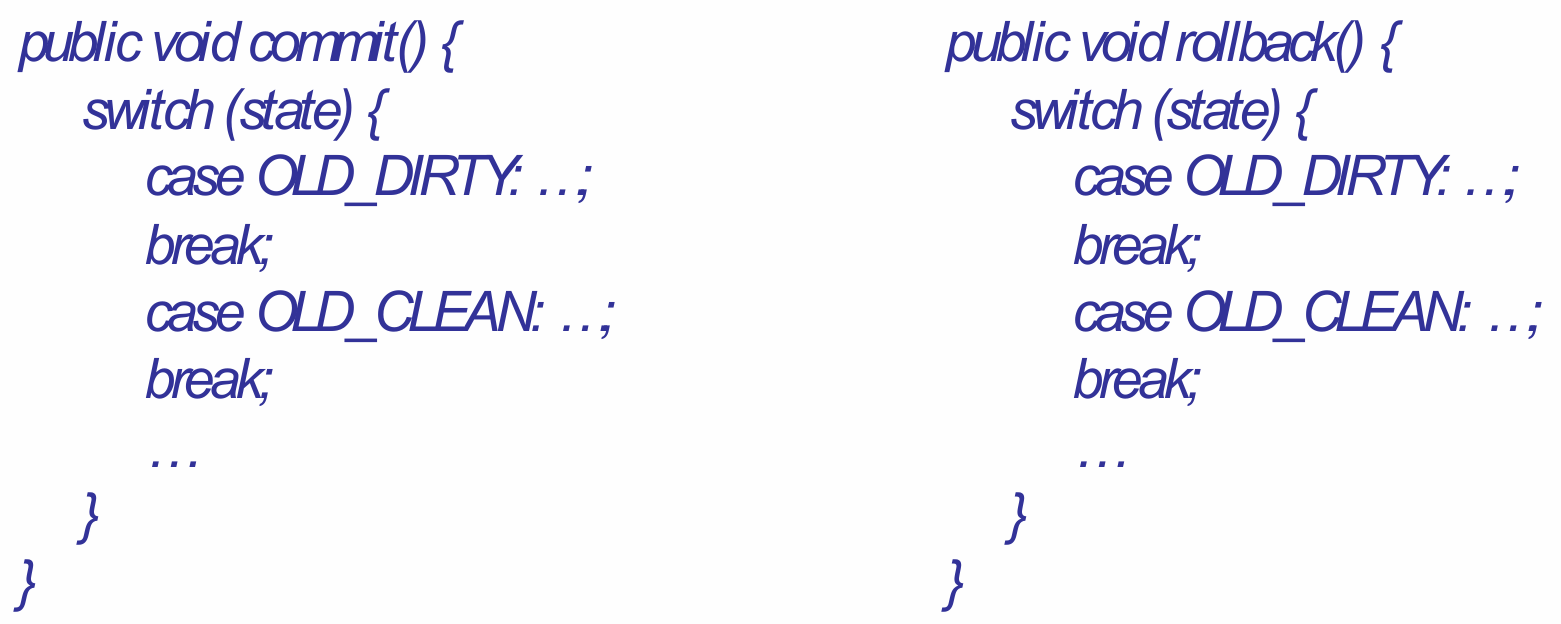
\includegraphics[scale=0.25]{Esercitazione - Design Patterns/Commit e Rollback.png}
    \end{center}
    Per evitare una ripetizione di codice, usiamo il pattern \textbf{State}:
    \begin{center}
        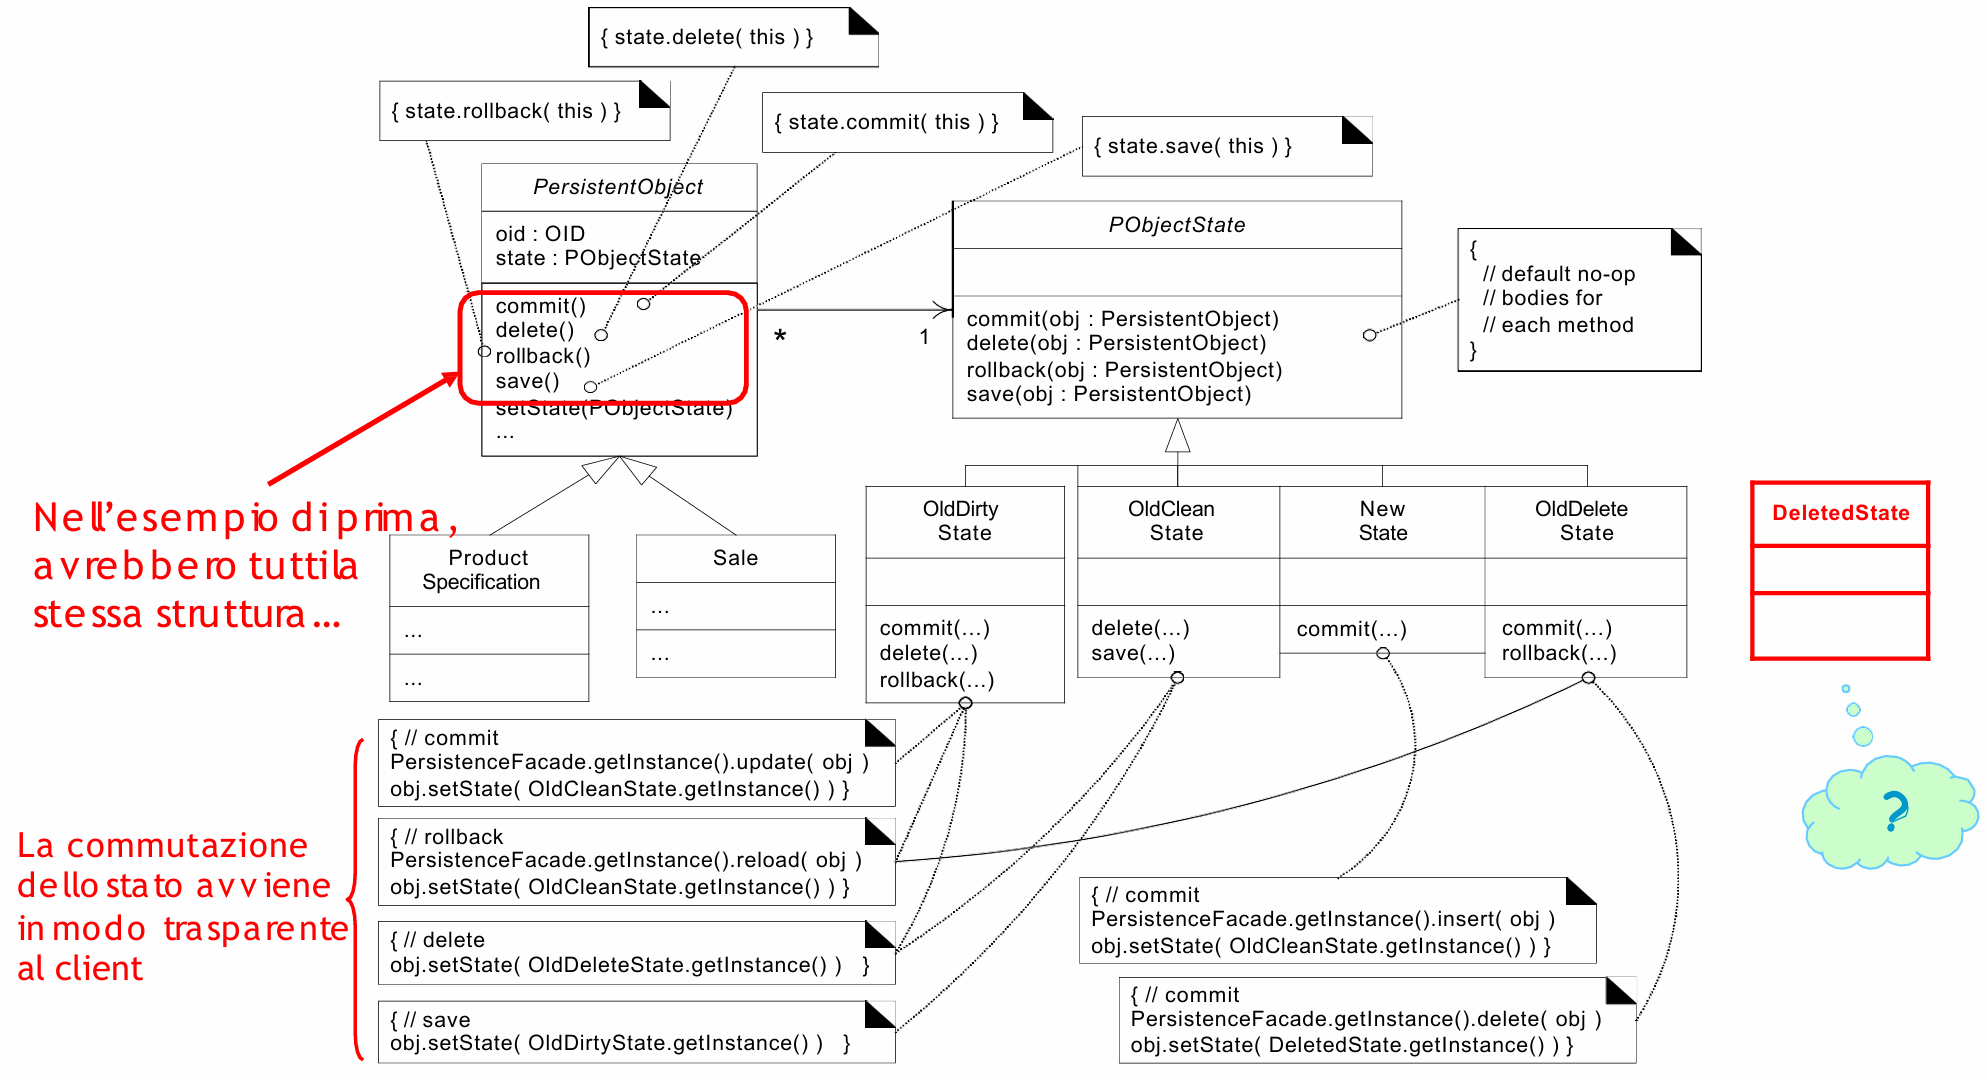
\includegraphics[scale=0.24]{Esercitazione - Design Patterns/State con Commit e Rollback.png}
    \end{center}
    Ricordando cosa fa lo State, crea delle classi che indicano gli stati, le classi implementano un'interfaccia
    comune. Questa interfaccia delega le operazioni all'oggetto \textbf{contesto} in base al suo stato corrente.

    Nell'esempio sopra il \textit{PersistentObject} rappresenta l'oggetto \textbf{Context}, mentre \textit{PObjectState}
    l'interfaccia \textbf{\textit{State}}. Per ogni stato concreto, definiamo le operazioni appropriate.
    \newpage
    \mysubsubsectionformatted{Modellazione delle operazioni di una transazione}
    Le transazioni, ovviamente, possono essere molteplici. In base all'ordine in cui vengono eseguite le operazioni all'interno
    di una transazione, si può influenzare la performance della transazione. Bisogna quindi trovare una soluzione, ovvero un modo
    per poter riordinare tutte le operazioni uguali prima di essere eseguiti. In questo ambito, interviene il pattern \textbf{Command}.
    
    Ricordando cosa fa Command, definisce per ciascun compito una classe che implementa un'interfaccia comune, a differenza di State che
    rappresentava uno stato, \textbf{nel Command ciascuna classe rappresenta un comando} e le azioni diventano oggetti.
    \begin{center}
        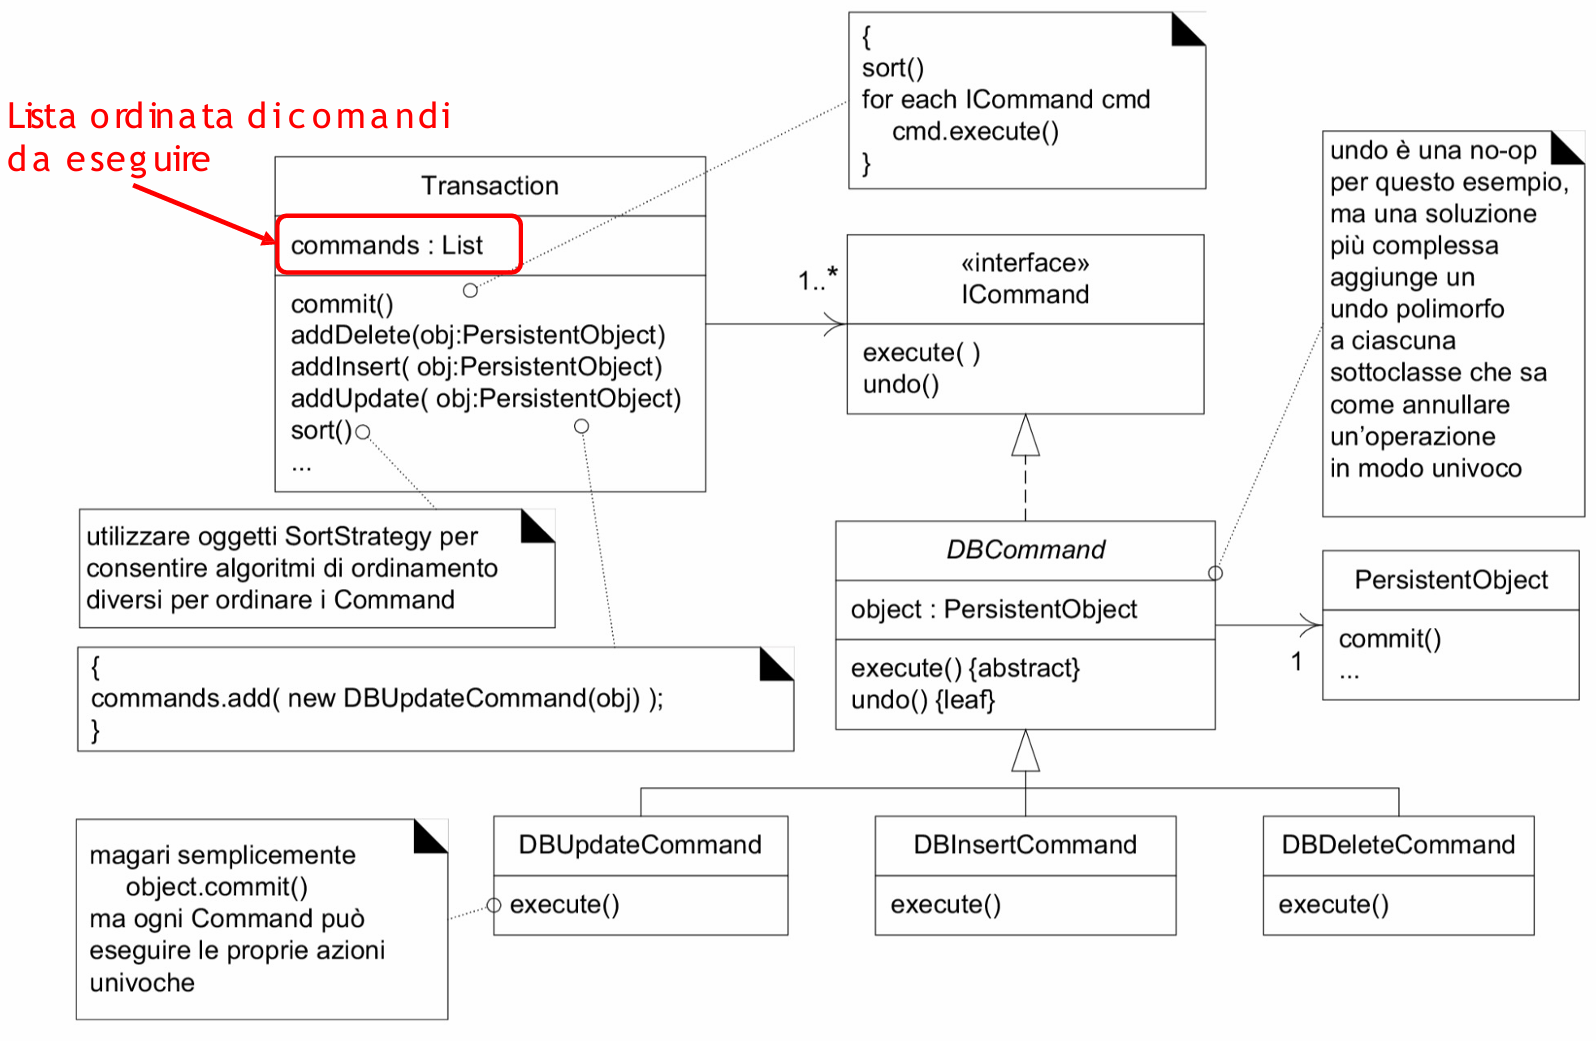
\includegraphics[scale=0.24]{Esercitazione - Design Patterns/Command con Commit e Rollback.png}
    \end{center}
    Nell'esempio, la classe Transaction è l'\textbf{invoker}, ovvero la classe che richiede all'interfaccia \textit{\textbf{ICommand}} le
    operazioni da eseguire. L'interfaccia riceve le operazioni e la classe DBCommand (la \textbf{ConcreteCommand}) incapsula le operazioni, per
    poi farle eseguire dal \textbf{Receiver}, ovvero la PersistentObject.
    \newpage
    \mysubsubsectionformatted{Lazy materialization con l'uso di Proxy}
    Ricordando la definizione di materializzazione, si tratta della traduzione di un record di un DB a un oggetto.

    A volte si vuole evitare il processo di materializzazione, per questioni di performance e a meno che non sia strettamente necessario. Si può
    risolvere questo problema tramite un processo di materializzazione "ritardata", ovvero la \textit{Lazy Materialization}.

    Il pattern utile allo scopo è il \coloredtext[blue]{\textbf{Virtual Proxy}}.
    \mysubsubsectionformatted{Design Pattern Virtual Proxy}
    \myparagraph{
    \begin{tcolorbox}[colback=blue!5!white, colframe=blue!75!black]
        Il Virtual Proxy è un Proxy per l'oggetto "reale", questo proxy virtuale
        materializza l'oggetto solo la prima volta a cui gli si fa riferimento,
        rappresentandoli come oggetti leggeri che fungono da sostituto all'oggetto
        reale (che possono essere più pesanti).
    \end{tcolorbox}

    In sostanza, il Virtual Proxy funge da sostituto dell'oggetto reale, ma in un formato
    più leggero. Sarà questo sostituto a gestire l'accesso all'oggetto reale e a caricarlo
    in memoria solo quando è strettamente necessario, in modo da evitare materializzazioni
    inutili.

    \begin{wrapfigure}{r}{0.55\textwidth}
        \begin{center}
          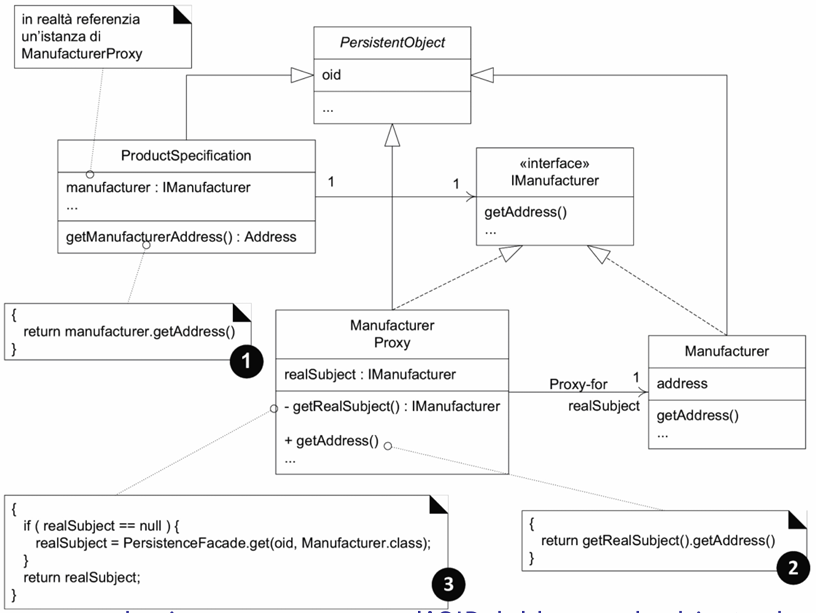
\includegraphics[width=0.55\textwidth]{Esercitazione - Design Patterns/Virtual Proxy.png}
        \end{center}
      \end{wrapfigure}
    
    \hbadness=2000
    Nell'esempio, Manufacturer è il nostro oggetto reale, \textbf{Manufacturer Proxy} è il suo \textbf{Virtual Proxy}, quindi
    un suo sostituto che ne gestisce l'accesso e stabilisce se caricarlo in memoria o meno. L'interfaccia comune \textit{IManufacturer}
    permette al client di interagire con il Virtual Proxy senza sapere che si tratta di un suo sostituto.

    Bisogna fare una considerazione, dato che parliamo di materializzazione ovviamente è coinvolto anche il pattern \textbf{DatabaseMapper},
    che in questo esempio è rappresentato dalla classe \textbf{ProductSpecification}, infatti questa crea un'istanza di \textit{IManufacturer},
    con lo scopo di decidere quali oggetti materializzare subito e a quali invece può ritardare questo processo. Si parla quindi di
    \textbf{Eager} e \textbf{Lazy Materialization}.

    \newpage
}
    \newpage
    \mysubsubsectionformatted{Eager vs Lazy Materialization}
\begin{center}
    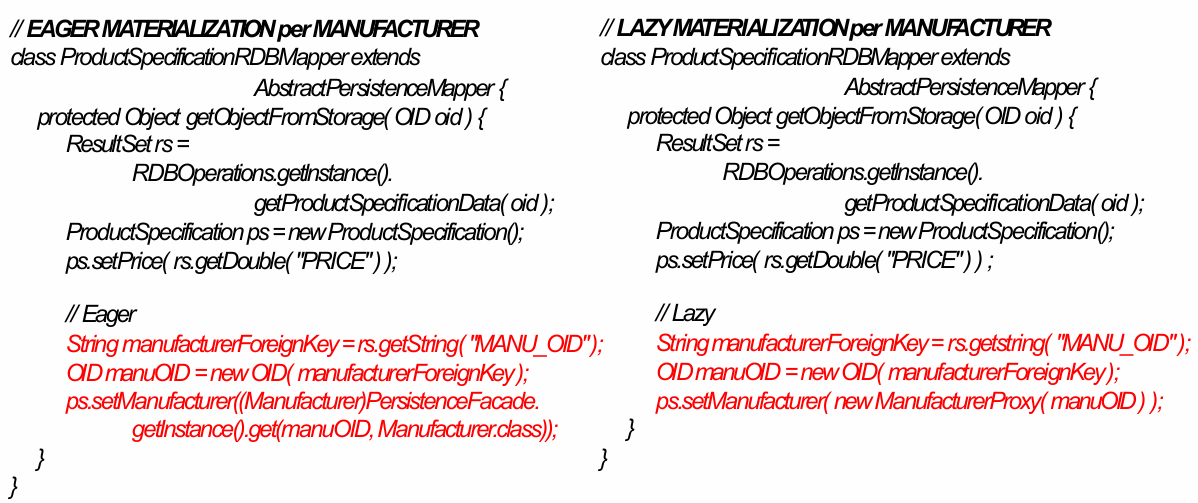
\includegraphics[scale=0.4]{Esercitazione - Design Patterns/Eager vs Lazy Materialization.png}
\end{center}

La differenza tra i due approcci sta nel caricamento in memoria del record in oggetto. Nel primo caso, avviene immediatamente
non appena i dati richiesti sono necessari, nel secondo caso il caricamento viene ritardato fino a quando l'oggetto non è
strettamente necessario.

Guardando il codice, entrambi gli approcci iniziano col prelevare la chiave\\ esterna del manifacturer, per poi creare un'ID da
associare all'oggetto (che verrà caricato in memoria) di quella chiave esterna (materializzazione: da record a oggetto).

\begin{enumerate}
    \item L'approccio \textbf{Eager} preleva direttamente l'oggetto Manufacturer \\dal database (\dots get(manuOID, Manufacturer.class))
    per poi settarlo al\\ Manufacturer oggetto.
    \item L'approccio \textbf{Lazy} agisce diversamente, crea prima un Virtual Proxy (ManufacturerProxy) dotato di identificativo
    unico (manuOID), settandolo nell'istanza di Manufacturer (ps). ManufacturerProxy rappresenta il sostituto di Manufacturer
    ma in formato più leggero e senza caricarlo in memoria direttamente.
\end{enumerate}
    
    }